\begin{exercise}
Für $i \in I$ sei $(X_i, \mathcal{T}_i)$ ein lokalkonvexer Vektorraum und
$\{p_{ij} ~|~ j \in J\}$ eine Familie von Seminormen, die $\mathcal{T}_i$ erzeugt.
Finde eine Familie von Seminormen auf $\prod_{i \in I} X_i$, welche die Produkttopologie erzeugt.

\end{exercise}

\begin{solution}



Wir identifizieren den Produktraum als Menge aller Auswahlfunktionen:
\begin{align*}
    \prod_{i \in I} X_i = \{f: I \rightarrow \bigcup_{i \in I} X_i ~|~ f(i) \in X_i\}.
\end{align*}

Auf dieser Menge definieren wir eine Familie von Seminormen:
\begin{align*}
    p_{ij}'(f) := p_{ij}(f(i)).
\end{align*}

$p_{ij}'$ ist eine Seminorm auf dem Produktraum:

\begin{itemize}
    \item $p_{ij}'(\alpha f) = p_{ij}(\alpha f(i)) = |\alpha|~ p_{ij}(f(i)) = |\alpha|~ p_{ij}'(f),$

    \item $p_{ij}'(f + g) = p_{ij}(f(i) + g(i)) \leq p_{ij}(f(i)) + p_{ij}(g(i)) = p_{ij}'(f) + p_{ij}'(g).$
\end{itemize}

Die Familie $(p_{ij}')_{(i,j) \in I \times J}$ ist überdies separierend: Seien $f, g \in \prod_{i \in I} X_i$ mit $f \neq g$. Dann existiert ein $i \in I$, sodass $g(i) \neq f(i)$. Für $g(i), f(i) \in X_i$ gibt es nun, weil die Familie $(p_{ij})_{j \in J}$ separierend ist, ein $j \in J$, sodass $p_{ij}(g(i)) \neq p_{ij}(f(i))$, was äquivalent zu $p_{ij}'(f) \neq p_{ij}'(g)$ ist.

Die durch die Familie der Seminormen $(p_{ij}')_{(i,j) \in I \times J}$ induzierte Topologie auf dem Produktraum ist die Initialtopologie der zugehörigen Projektionen $(\pi_{ij}')_{(i,j) \in I \times J}:$

\begin{align*}
  \pi_{ij}':
  ~\begin{cases}
    \prod_{i \in I} X_i \rightarrow (\prod_{i \in I} X_i) / N(p_{ij}')\\
    f \mapsto f + N(p_{ij}'), \text{wobei}~ N(p_{ij}') := \{g \in \prod_{i \in I} X_i ~|~ p_{ij}'(g) = 0\}.
  \end{cases}
\end{align*}

Jeder Faktorraum $(\prod_{i \in I} X_i) / N(p_{ij}')$ trägt dabei jene Topologie, die von der Norm $\overline{p_{ij}'}$ induziert wird,
welche repräsentantenweise durch die Seminorm ${p_{ij}'}$ definiert ist.

Eine Basis der Topologie im Produktraum bezüglich der von den Seminormen induzierten Topologie bildet folgende Menge:
\begin{align*}
    \mathcal{B} =
    \{\bigcap_{(i,j) \in E} (\pi_{ij}')^{-1}(U^{{\overline{p_{ij}'}}}_{\epsilon_{ij}}(x_{ij} + N(p_{ij}'))
    ~|~ \epsilon_{ij} > 0, E \subset I \times J : |E| < \infty
    \}.
\end{align*}

Es gilt
\begin{align*}
    (\pi_{ij}')^{-1}(U^{{\overline{p_{ij}'}}}_{\epsilon_{ij}}x_{ij} + (N(p_{ij}')))
   = \{ f \in \prod_{i \in I} X_i ~|~
   \overline{p_{ij}'}(\pi_{ij}'(f) - x_{ij} + N(p_{ij}'))
   < \epsilon_{ij} \}
   = \{ f \in \prod_{i \in I} X_i ~|~
   p_{ij}'(f) < \epsilon \}
   = U_{\epsilon_{ij}}^{p_{ij}'}(x_{ij}),
\end{align*}

eine Basis der Topologie besteht also genau aus den endlichen Schnitten von Kugeln bezüglich der Seminormen.


Betrachten wir nun eine Basis der Produkttopologie:

\begin{align*}
    \mathcal{C} =
    \{\bigcap_{i \in E} (\pi_{i})^{-1}(V_i)
    ~|~ V_i \in \mathcal{T}_i, E \subset I: |E| < \infty
    \}.
\end{align*}

Die Räume $(X_i, \mathcal{T}_i)$ sind nun ihrerseits wiederum von den Familien
$\{p_{ij} ~|~ j \in J\}$ von Seminormen erzeugt. Jedes V aus der oberen Menge enthält also einen endlichen Schnitt von Kugeln:
\begin{align*}
 \bigcap_{j \in E} U_{\epsilon}^{p_{ij}}(x_j) \subseteq V.
\end{align*}

Demnach lassen sich die Mengen aus $\mathcal{C}$ schreiben als

\begin{align*}
    \bigcap_{i \in E_1} (\pi_{i})^{-1}(\bigcap_{j \in E_2} U_{\epsilon}^{p_{ij}}(x_j))
    =
    \bigcap_{i \in E_1}
    \bigcap_{j \in E_2}
    (\pi_{i})^{-1}(U_{\epsilon}^{p_{ij}}(x_j))
    =
    \bigcap_{(i,j) \in E_1 \times E_2} U_{\epsilon}^{p_{ij}'}(x_j);
\end{align*}

insgesamt gilt also $\mathcal{B} = \mathcal{C}$, was zu zeigen war.

****************

Wir betrachten $K := \Bbraces{(i,j) \mid i \in I \land j \in J_i}$ und die Familie
\begin{align*}
    M := (p_{ik} \circ \pi_i \mid \prod_{i \in I} X_i \to [0, \infty))_{(i, k) \in K}
\end{align*}
von Seminormen. Dies entspricht genau den Abbildungen oben, wo mit Auswahlfunktionen gearbeitet wurde, dort sieht man, dass es sich um Seminormen handelt und die Menge $M$ separierend ist. Nach Satz 5.1.4 erhalten wir mit der Initialtopologie bezüglich der Familie $M$ also einen lokalkonvexen topologischen Vektorraum auf dem Produktraum. Wir haben die Funktionen
\begin{align*}
    \pi_{p_{kn} \circ \pi_k}: \prod_{i \in I} X_i \to \prod_{i \in I} X_i /_{N(p_{kn} \circ \pi_k)}: (x_i)_{i \in I} \mapsto (x_i)_{i \in I} + N(p_{kn} \circ \pi_k) 
\end{align*}

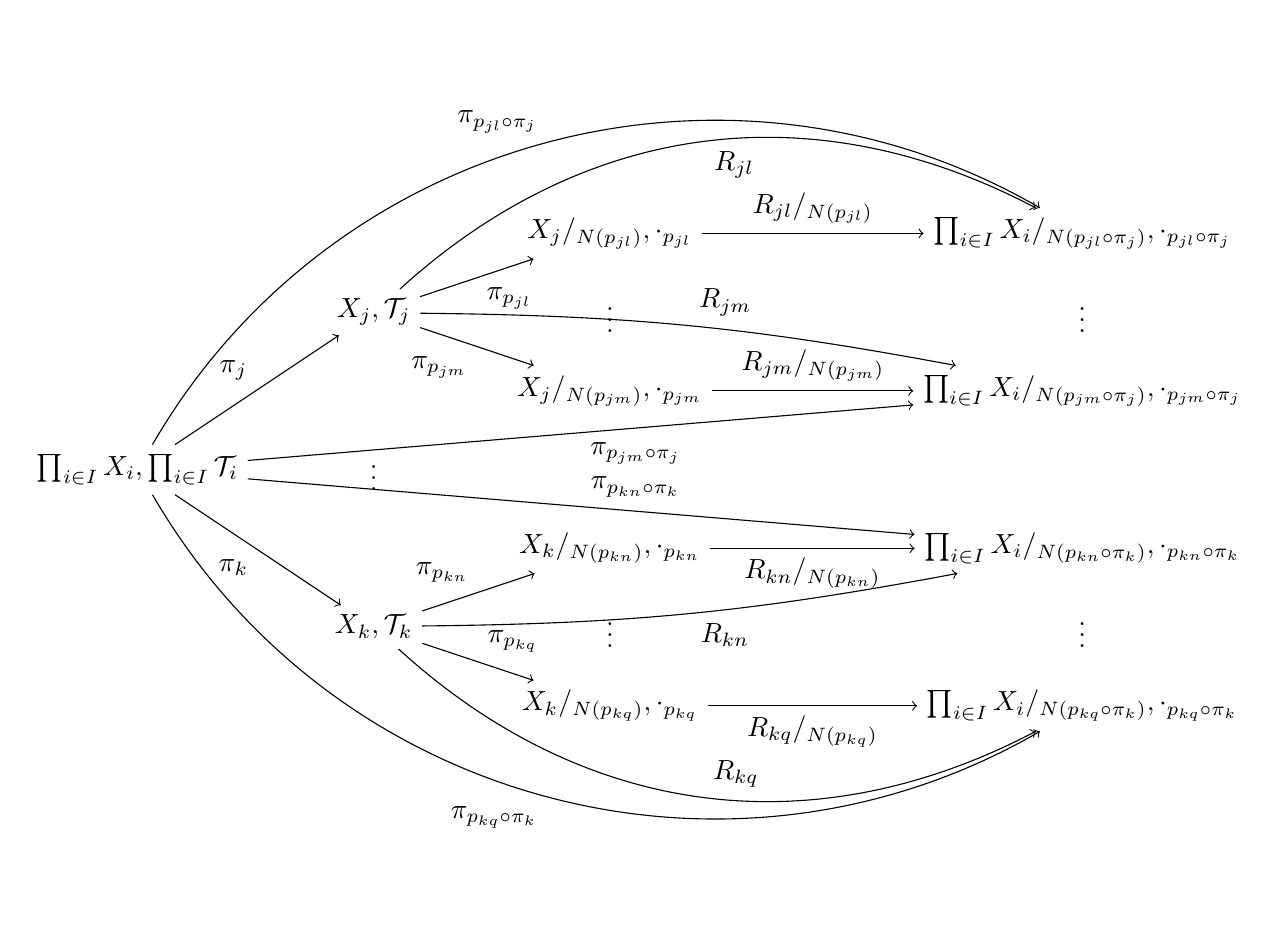
\begin{tikzpicture}[auto]
    \node (prod) at (0,0) {$\pbraces{\prod_{i \in I} X_i, \prod_{i \in I} \mathcal{T}_i }$};

    \node (xj) at (3,2) {$\pbraces{X_j, \mathcal{T}_j}$};
    \node (dots1) at (3,0) {$\vdots$};
    \node (xk) at (3,-2) {$\pbraces{X_k, \mathcal{T}_k}$};

    \node (xj_fac_l) at (6,3) {$\pbraces{X_j/_{N(p_{jl})}, \norm{\cdot}{_{p_{jl}}}}$};
    \node (dots2) at (6, 2) {$\vdots$};
    \node (xj_fac_m) at (6,1) {$\pbraces{X_j/_{N(p_{jm})}, \norm{\cdot}{_{p_{jm}}}}$};

    \node (xk_fac_n) at (6,-1) {$\pbraces{X_k/_{N(p_{kn})}, \norm{\cdot}{_{p_{kn}}}}$};
    \node (dots3) at (6, -2) {$\vdots$};
    \node (xk_fac_q) at (6,-3) {$\pbraces{X_k/_{N(p_{kq})}, \norm{\cdot}{_{p_{kq}}}}$};

    \node (prod_fac_jl) at (12,3) {$\pbraces{\prod_{i \in I} X_i/_{N(p_{jl} \circ \pi_j)}, \norm{\cdot}{_{p_{jl} \circ \pi_j}}}$};
    \node (dots4) at (12,2) {$\vdots$};
    \node (prod_fac_jm) at (12,1) {$\pbraces{\prod_{i \in I} X_i/_{N(p_{jm} \circ \pi_j)}, \norm{\cdot}{_{p_{jm} \circ \pi_j}}}$};

    \node (prod_fac_kn) at (12,-1) {$\pbraces{\prod_{i \in I} X_i/_{N(p_{kn} \circ \pi_k)}, \norm{\cdot}{_{p_{kn} \circ \pi_k}}}$};
    \node (dots5) at (12, -2) {$\vdots$};
    \node (prod_fac_kq) at (12,-3) {$\pbraces{\prod_{i \in I} X_i/_{N(p_{kq} \circ \pi_k)}, \norm{\cdot}{_{p_{kq} \circ \pi_k}}}$};

    \draw[->] (prod) to node {$\pi_j$} (xj);
    \draw[->] (prod) to node [swap] {$\pi_k$} (xk);

    \draw[->] (xj) to node[swap] {$\pi_{p_{jl}}$} (xj_fac_l);
    \draw[->] (xj) to node [swap] {$\pi_{p_{jm}}$} (xj_fac_m);

    \draw[->] (xk) to node {$\pi_{p_{kn}}$} (xk_fac_n);
    \draw[->] (xk) to node {$\pi_{p_{kq}}$} (xk_fac_q);

    \draw[->, bend left = 45] (prod) to node {$\pi_{p_{jl} \circ \pi_j} $} (prod_fac_jl);
    \draw[->] (prod) to node[swap] {$\pi_{p_{jm} \circ \pi_j} $} (prod_fac_jm);
    \draw[->] (prod) to node {$\pi_{p_{kn} \circ \pi_k} $} (prod_fac_kn);
    \draw[->, bend right = 45] (prod) to node[swap] {$\pi_{p_{kq} \circ \pi_k} $} (prod_fac_kq);

    \draw[->, bend left = 35] (xj) to node[swap] {$R_{jl}$} (prod_fac_jl);
    \draw[->, bend left = 5] (xj) to node {$R_{jm}$} (prod_fac_jm);
    \draw[->, bend right = 5] (xk) to node[swap] {$R_{kn}$} (prod_fac_kn);
    \draw[->, bend right = 35] (xk) to node {$R_{kq}$} (prod_fac_kq);

    \draw[->] (xj_fac_l) to node {$R_{jl}/_{N(p_{jl})}$} (prod_fac_jl);
    \draw[->] (xj_fac_m) to node {$R_{jm}/_{N(p_{jm})}$} (prod_fac_jm);
    \draw[->] (xk_fac_n) to node[swap] {$R_{kn}/_{N(p_{kn})}$} (prod_fac_kn);
    \draw[->] (xk_fac_q) to node[swap] {$R_{kq}/_{N(p_{kq})}$} (prod_fac_kq);
\end{tikzpicture}

Für alle $k \in I$ und $n \in J_k$ ist
\begin{align*}
    R_{kn}: X_k \to \prod_{i \in I} X_i /_{N(p_{kn} \circ \pi_k)}: x \mapsto (x_i)_{i \in I} + N(p_{kn} \circ \pi_k) \quad \textrm{mit} \quad x_k = x
\end{align*}
linear und surjektiv mit
\begin{align*}
    \bigcap_{j \in J_k} \ker R_{kj} = {0}.
\end{align*}
Gemäß Bemerkung 5.1.6 ist
\begin{align*}
    R_{kn}/_{N(p_{kn})}: X_k/_{N(p_{kn})} \to \prod_{i \in I} X_i /_{N(p_{kn} \circ \pi_k)}: x + N(p_{kn}) \mapsto (x_i)_{i \in I} + N(p_{kn} \circ \pi_k) \quad \textrm{mit} \quad x_k = x
\end{align*}
ein Homöomorphismus, welcher glücklicherweise
\begin{align*}
    R_{kn} = R_{kn}/_{N(p_{kn})} \circ \pi_{p_{kn}}
\end{align*}
 erfüllt, also ist $\mathcal{T}_k$ die initiale Topologie bezüglich der $(R_{kj})_{j \in J_k}$. Nun gilt aber glücklicherweise auch 
 \begin{align*}
     \pi_{p_{kn} \circ \pi_k} = R_{kn} \circ \pi_k
 \end{align*}
 also sind wir mit Korollar 1.2.4 fertig.

\end{solution}
